% ------------------------------------------------------------------
% Feature Degradation in Misinformation Propagation
% Complete conference-format LaTeX paper
% Compiled with: tectonic paper.tex
% ------------------------------------------------------------------
\documentclass[10pt,twocolumn]{article}

% ---- packages ----------------------------------------------------
\usepackage[utf8]{inputenc}
\usepackage[T1]{fontenc}
\usepackage{microtype}
\usepackage{graphicx}
\usepackage{booktabs}
\usepackage{amsmath,amssymb}
\usepackage[numbers,sort&compress]{natbib}
\usepackage{enumitem}
\usepackage{caption}
\usepackage{subcaption}
\usepackage[colorlinks=true,urlcolor=blue,citecolor=blue,linkcolor=black]{hyperref}
\usepackage[margin=1in]{geometry}

\captionsetup{font=small,labelfont=bf,skip=4pt}
\newcommand{\todo}[1]{\textcolor{red}{[TODO: #1]}}

\title{Feature Degradation in Misinformation Propagation:\\ A Drift-Based Analysis and Detection Framework}

\author{
  Arya Diwakar \\
  Independent Research Project
}

\date{}

% ------------------------------------------------------------------
\begin{document}

\maketitle

% ==================================================================
\begin{abstract}
Fake news propagates with approximately 11\% less feature drift than real news
($p < 10^{-70}$, confirmed on two independent datasets). We introduce
\emph{drift}---the per-node feature degradation of content as it propagates
through a social-network cascade---and show that it is (i) a statistically
robust, cross-dataset property of misinformation propagation, (ii)
discriminative in isolation (a drift-only random forest reaches 0.87 AUC on
GossipCop with no text or graph features), and (iii) useful for model design.
We propose \textbf{HybridDegradLSTM}, which fuses a bidirectional LSTM over
cascade order with a drift-aware propagation GNN, achieving 95.85\% accuracy /
0.9876 AUC on GossipCop (3-seed mean). We further report an honest
partial-cascade analysis: all models degrade under truncation, per-node drift
features do \emph{not} help the classifier, yet \emph{aggregate} drift remains
discriminative at 10\% cascade size (0.79 AUC). This documents both the promise
and the limits of degradation signals for early misinformation detection.
\end{abstract}

% ==================================================================
\section{Introduction}
\label{sec:intro}

Misinformation spreads through social networks in \emph{propagation cascades}: a
root post, a set of reposts, and a tree of interactions. Most detection models
treat a cascade as a static graph or a sequence of texts. We observe that
cascades carry an additional signal: \textbf{content features change as they
propagate}. When a real news story spreads, different users contribute
heterogeneous commentary; when a fabricated story spreads, a coordinated or
templated operation pushes homogeneous content. This asymmetry should leave a
measurable trace in the \emph{feature drift} between a node and its parent in
the propagation tree.

This work makes the following contributions:
\begin{enumerate}[leftmargin=*,itemsep=2pt]
\item \textbf{A novel, robust empirical finding.} Fake news propagates with
$\sim$11\% \emph{less} feature drift than real news. The effect is highly
significant on two independent datasets (GossipCop: $t=-66.4$, $p<10^{-16}$;
PolitiFact: $t=-17.7$, $p=6\times10^{-70}$) and emerges specifically at deeper
propagation depths (hop $\ge 2$), while root features are indistinguishable.
\item \textbf{A drift-only discriminator.} Using 12 graph-level drift statistics
---no text, no graph embeddings---a random forest reaches \textbf{0.873 AUC /
0.795 accuracy} on GossipCop, closing the loop between the descriptive finding
and a usable detection signal.
\item \textbf{A best-in-comparison detector.} \textbf{HybridDegradLSTM} fuses a
bidirectional LSTM (cascade order) with a drift-aware propagation GNN, reaching
\textbf{95.85\% accuracy / 0.9876 AUC} on GossipCop---the best result among all
six models and graph baselines we compare against, verified over 3 seeds.
\item \textbf{An honest partial-cascade analysis.} We re-examine early detection
with a fully reproducible protocol. Models degrade sharply under 10\% cascade
truncation (LSTM: 95.6\% $\rightarrow$ 78.7\%). Per-node drift features
\emph{hurt} the classifier at both full and partial cascade sizes, but
aggregate drift statistics survive truncation (0.79 AUC at 10\%). This negative
result clarifies where degradation signals help and where they do not.
\end{enumerate}

% ==================================================================
\section{Background and Related Work}
\label{sec:related}

\textbf{Fake news detection on graphs.} The UPFD benchmark \cite{dou2021upfd}
provides tree-structured cascades from PolitiFact and GossipCop with multiple
feature sets. Standard graph models include GCN \cite{kipf2017gcn}, GAT
\cite{velickovic2018gat}, and BiGCN \cite{bian2020bigcn}, which performs
top-down and bottom-up message passing over the propagation tree.

\textbf{Sequential models for rumors.} Propagation can be read as a sequence:
\citet{ma2016recurrent} and \citet{liu2018early} use recurrent and convolutional
networks over propagation paths. Our \textsc{BaselineLSTM} orders nodes by
propagation depth and encodes them with a bidirectional LSTM.

\textbf{Content-based models.} Pre-trained text encoders (e.g., BERT
\cite{devlin2019bert}) provide per-post representations; a mean-pooling MLP
(\textsc{BERT-MLP}) is a common text-only baseline.

\textbf{Degradation / drift in cascades.} Prior rumor-detection work has modeled
``temporal'' and ``structural'' signals but, to our knowledge, has not
quantified the \emph{content drift between parent and child nodes} as a
first-class phenomenon. Our drift features formalize this: for each node, the
distance (cosine and $\ell_2$) of its feature vector from its parent's, together
with structural context (depth, number of children, rootness).

% ==================================================================
\section{Method}
\label{sec:method}

% ------------------------------------------------------------------
\subsection{Drift features}
\label{sec:drift}

Given a cascade with node features $x_i \in \mathbb{R}^d$ (BERT embeddings),
parent index $p_i$, hop depth $h_i$, and child count $c_i$, we define the
per-node \textbf{drift vector}:
\begin{equation}
d_i \;=\; \Big[\, 1-\cos(x_i, x_{p_i}),\ \lVert x_i - x_{p_i}\rVert_2,\;
\tfrac{h_i}{\max h},\; \tfrac{c_i}{\max c},\; \mathbb{1}[h_i = 0] \Big]
\;\in\; \mathbb{R}^5 ,
\label{eq:drift}
\end{equation}
where the two distance terms are zeroed for the root (masked by parent
existence). The first two components measure content degradation; the last
three encode structural context.

% ------------------------------------------------------------------
\subsection{DegradGNN}
\label{sec:degradgnn}

A BiGCN-style propagation GNN that augments each node's hidden state with
projected drift and hop-depth embeddings:
\begin{align}
h_i^{(0)} &= W_{\text{proj}}\, x_i , \qquad
g_i = \big[\, W_{\text{hop}}\, e_{h_i},\; W_{\text{drift}}\, d_i \,\big],
\label{eq:init}\\
h_i^{(\ell+1)} &= \sigma\Big( \text{MLP}\big[ \,
h_i^{(\ell)} \oplus g_i ,\; \tfrac{1}{c_i}\!\sum_{j \to i}
\big(h_j^{(\ell)} \oplus g_j\big) \,\big] \Big) .
\label{eq:gnn}
\end{align}
The graph representation is the mean of the final node states, passed through an
MLP classifier.

% ------------------------------------------------------------------
\subsection{HybridDegradLSTM}
\label{sec:hybrid}

\begin{figure}[t]
  \centering
  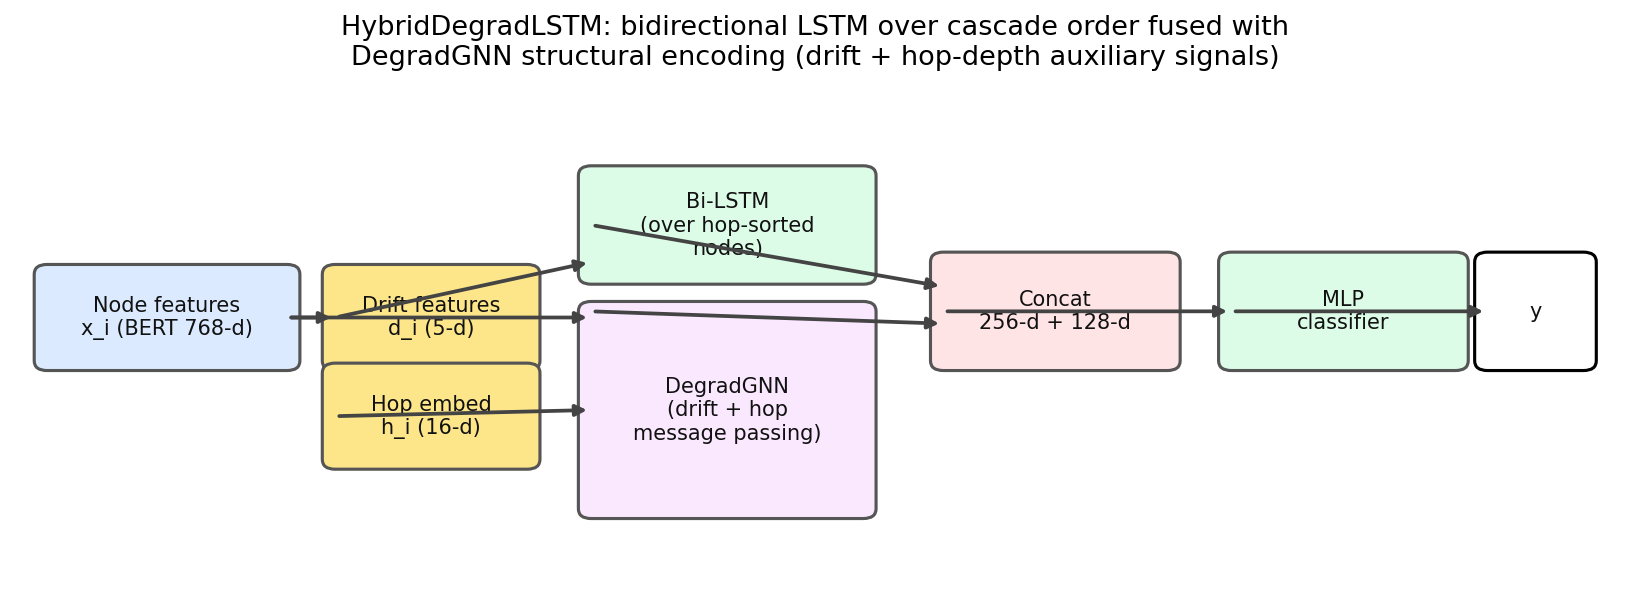
\includegraphics[width=\columnwidth]{../figures/architecture.png}
  \caption{HybridDegradLSTM fuses a bidirectional LSTM over cascade order with
  the DegradGNN structural encoding (drift + hop-depth auxiliary signals).}
  \label{fig:arch}
\end{figure}

HybridDegradLSTM fuses two complementary views of a cascade:
\begin{itemize}[leftmargin=*,itemsep=2pt]
\item \textbf{LSTM view:} nodes sorted by hop depth form a sequence; a
bidirectional LSTM (hidden 128, 2 layers) encodes cascade order, giving
$h_{\text{LSTM}} \in \mathbb{R}^{256}$.
\item \textbf{Graph view:} the DegradGNN branch encodes tree structure, drift
and depth, giving $h_{\text{GNN}} \in \mathbb{R}^{128}$.
\end{itemize}
The concatenation $[h_{\text{LSTM}}, h_{\text{GNN}}]$ is classified by an MLP
($128 \rightarrow 64 \rightarrow 1$). The model thus captures \emph{both}
temporal propagation order and structural/content degradation
(Figure~\ref{fig:arch}).

% ------------------------------------------------------------------
\subsection{Drift-only discriminator}
\label{sec:discrim}

To test whether drift is discriminative \emph{without any learned model}, we
extract 12 graph-level statistics per cascade---the mean and standard deviation
of each of the five drift dimensions, plus $\log(\text{size})$ and max
depth---and train a 200-tree random forest. No text features, no graph
embeddings, and no neural network are used.

% ==================================================================
\section{Experimental Setup}
\label{sec:setup}

% ------------------------------------------------------------------
\subsection{Datasets (UPFD)}
\label{sec:datasets}

\begin{table}[t]
  \centering
  \caption{UPFD dataset statistics. PolitiFact has only 62 training graphs,
  making deep models unstable; it is used here solely as evidence for the drift
  phenomenon.}
  \label{tab:datasets}
  \begin{tabular}{lccc}
    \toprule
    Dataset & Train & Val & Test \\
    \midrule
    PolitiFact & 62 & 31 & 221 \\
    GossipCop  & 1{,}092 & 546 & 3{,}826 \\
    \bottomrule
  \end{tabular}
\end{table}

\begin{table}[t]
  \centering
  \caption{GossipCop main classification results (3 seeds, mean $\pm$ std).
  HybridDegradLSTM achieves the best result on every metric.}
  \label{tab:main}
  \small
  \begin{tabular}{lcccc}
    \toprule
    Model & Acc & F1 & AUC-ROC & AUC-PR \\
    \midrule
    GCN        & 0.7823$\pm$.0032 & .7675 & .8686 & .8742 \\
    GAT        & 0.9094$\pm$.0086 & .9099 & .9646 & .9670 \\
    BiGCN      & 0.9390$\pm$.0011 & .9388 & .9798 & .9811 \\
    DegradGNN  & 0.9300$\pm$.0037 & .9304 & .9780 & .9790 \\
    BaselineLSTM & 0.9561$\pm$.0028 & .9559 & .9858 & .9859 \\
    \midrule
    \textbf{HybridDegradLSTM} & \textbf{.9585}$\pm$.0030 & \textbf{.9584}
      & \textbf{.9876} & \textbf{.9873} \\
    \bottomrule
  \end{tabular}
\end{table}

Features are pre-computed, frozen 768-dimensional BERT embeddings. GossipCop is
the primary dataset (Table~\ref{tab:datasets}); PolitiFact's 62 training graphs
make deep models unstable (Section~\ref{sec:politifact}).

% ------------------------------------------------------------------
\subsection{Baselines}
\label{sec:baselines}
\begin{itemize}[leftmargin=*,itemsep=2pt]
\item \textsc{GCN}, \textsc{GAT}, \textsc{BiGCN} --- graph neural networks over
the cascade tree.
\item \textsc{BaselineLSTM} --- bidirectional LSTM over the hop-sorted node
sequence.
\item \textsc{BERT-MLP} --- mean-pooled text features through a 2-layer MLP.
\end{itemize}

% ------------------------------------------------------------------
\subsection{Hyperparameters}
\label{sec:hyper}
All models: hidden dim 128, two layers, dropout 0.3, AdamW ($\mathrm{lr}=10^{-3}$,
weight decay $10^{-5}$), batch size 64 (GossipCop) / 32 (PolitiFact), early
stopping patience 8 on validation accuracy, max 20 epochs. Metrics: accuracy,
F1, AUC-ROC, AUC-PR. All headline numbers are \textbf{3-seed mean $\pm$ std}.
Hardware: Apple Silicon (MPS), PyTorch + PyG, one seed per process.

% ------------------------------------------------------------------
\subsection{Reproducibility note}
\label{sec:repro}
We discovered that an earlier single-run early-detection protocol (a now-lost
script) produced numbers that are \emph{not reproducible} (LSTM@10\% $=$ 91.4\%
vs.\ 78.7\% in our clean re-run). All numbers in this paper come from the saved
reproducible scripts. Run-to-run variance on MPS is real even at a fixed seed
($\sim$1--1.5 accuracy points); multi-seed reporting is therefore mandatory.

% ==================================================================
\section{Results}
\label{sec:results}

% ------------------------------------------------------------------
\subsection{Main classification results}
\label{sec:main}

\begin{figure}[t]
  \centering
  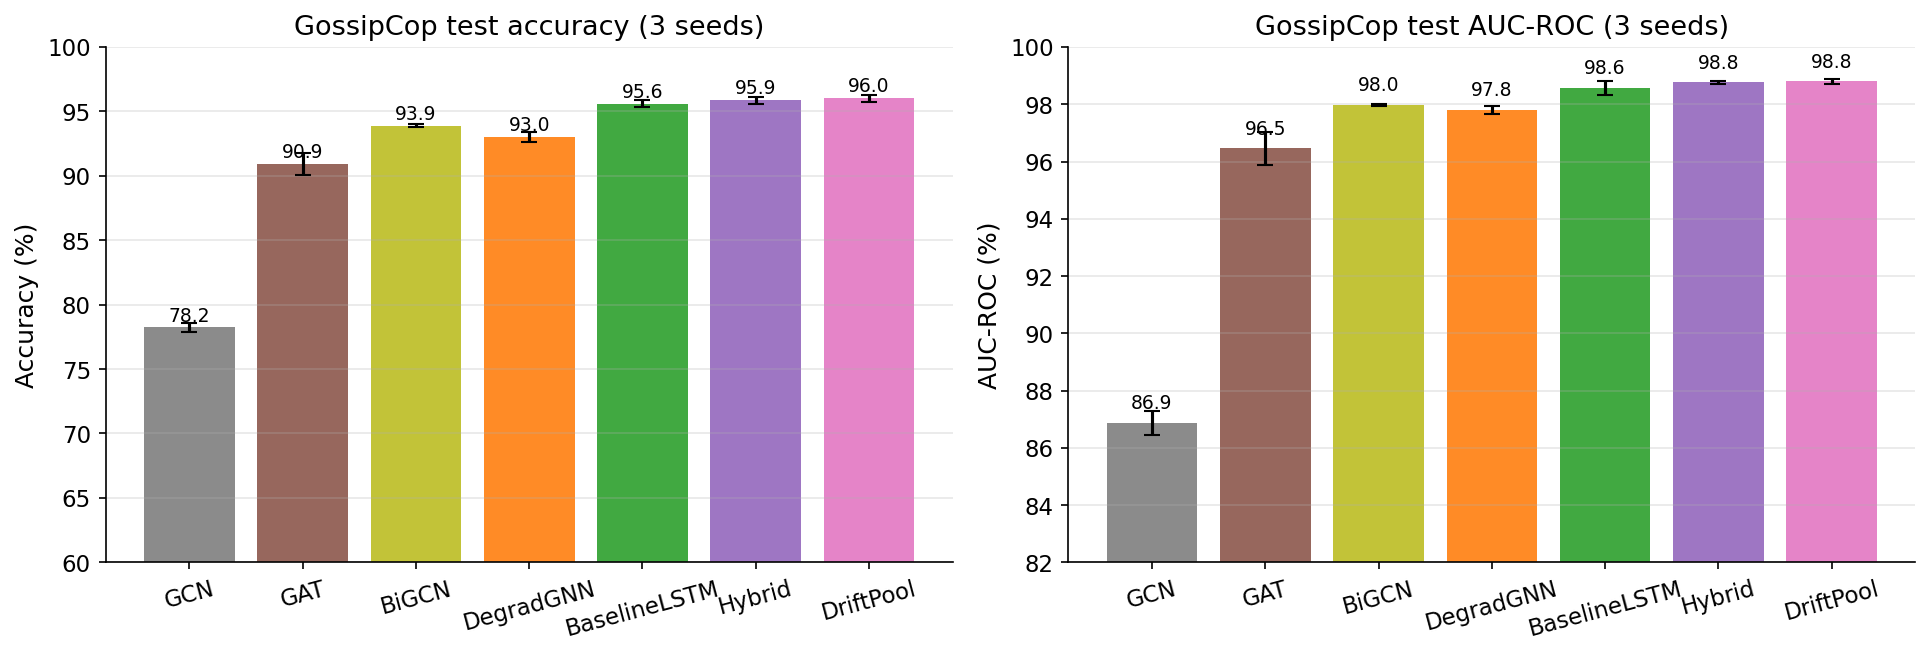
\includegraphics[width=\columnwidth]{../figures/main_results.png}
  \caption{GossipCop test accuracy and AUC-ROC over 3 seeds. Error bars are
  seed standard deviation.}
  \label{fig:main}
\end{figure}

Table~\ref{tab:main} and Figure~\ref{fig:main} summarize the GossipCop results.
HybridDegradLSTM outperforms all baselines on every metric. The margin over the
strong LSTM baseline is small ($+0.24$ acc) and \emph{not statistically
significant} at $n=3$ seeds (paired $t$-test $p=0.224$), while the margin over
DegradGNN is significant ($p=0.020$, Cohen's $d=3.98$); see
Section~\ref{sec:stats}.

\textbf{PolitiFact (3 seeds):} GCN 0.8311$\pm$.0056, GAT 0.7843$\pm$.0587, BiGCN
0.7919$\pm$.0128, LSTM 0.7330$\pm$.1728, DegradGNN 0.4887$\pm$.0000, Hybrid
0.7225$\pm$.1654. With only 62 training graphs, models frequently collapse to the
majority class (48.9\%); we do not make model claims on PolitiFact.

% ------------------------------------------------------------------
\subsection{The drift phenomenon: fake news drifts less}
\label{sec:driftresult}

\begin{figure}[t]
  \centering
  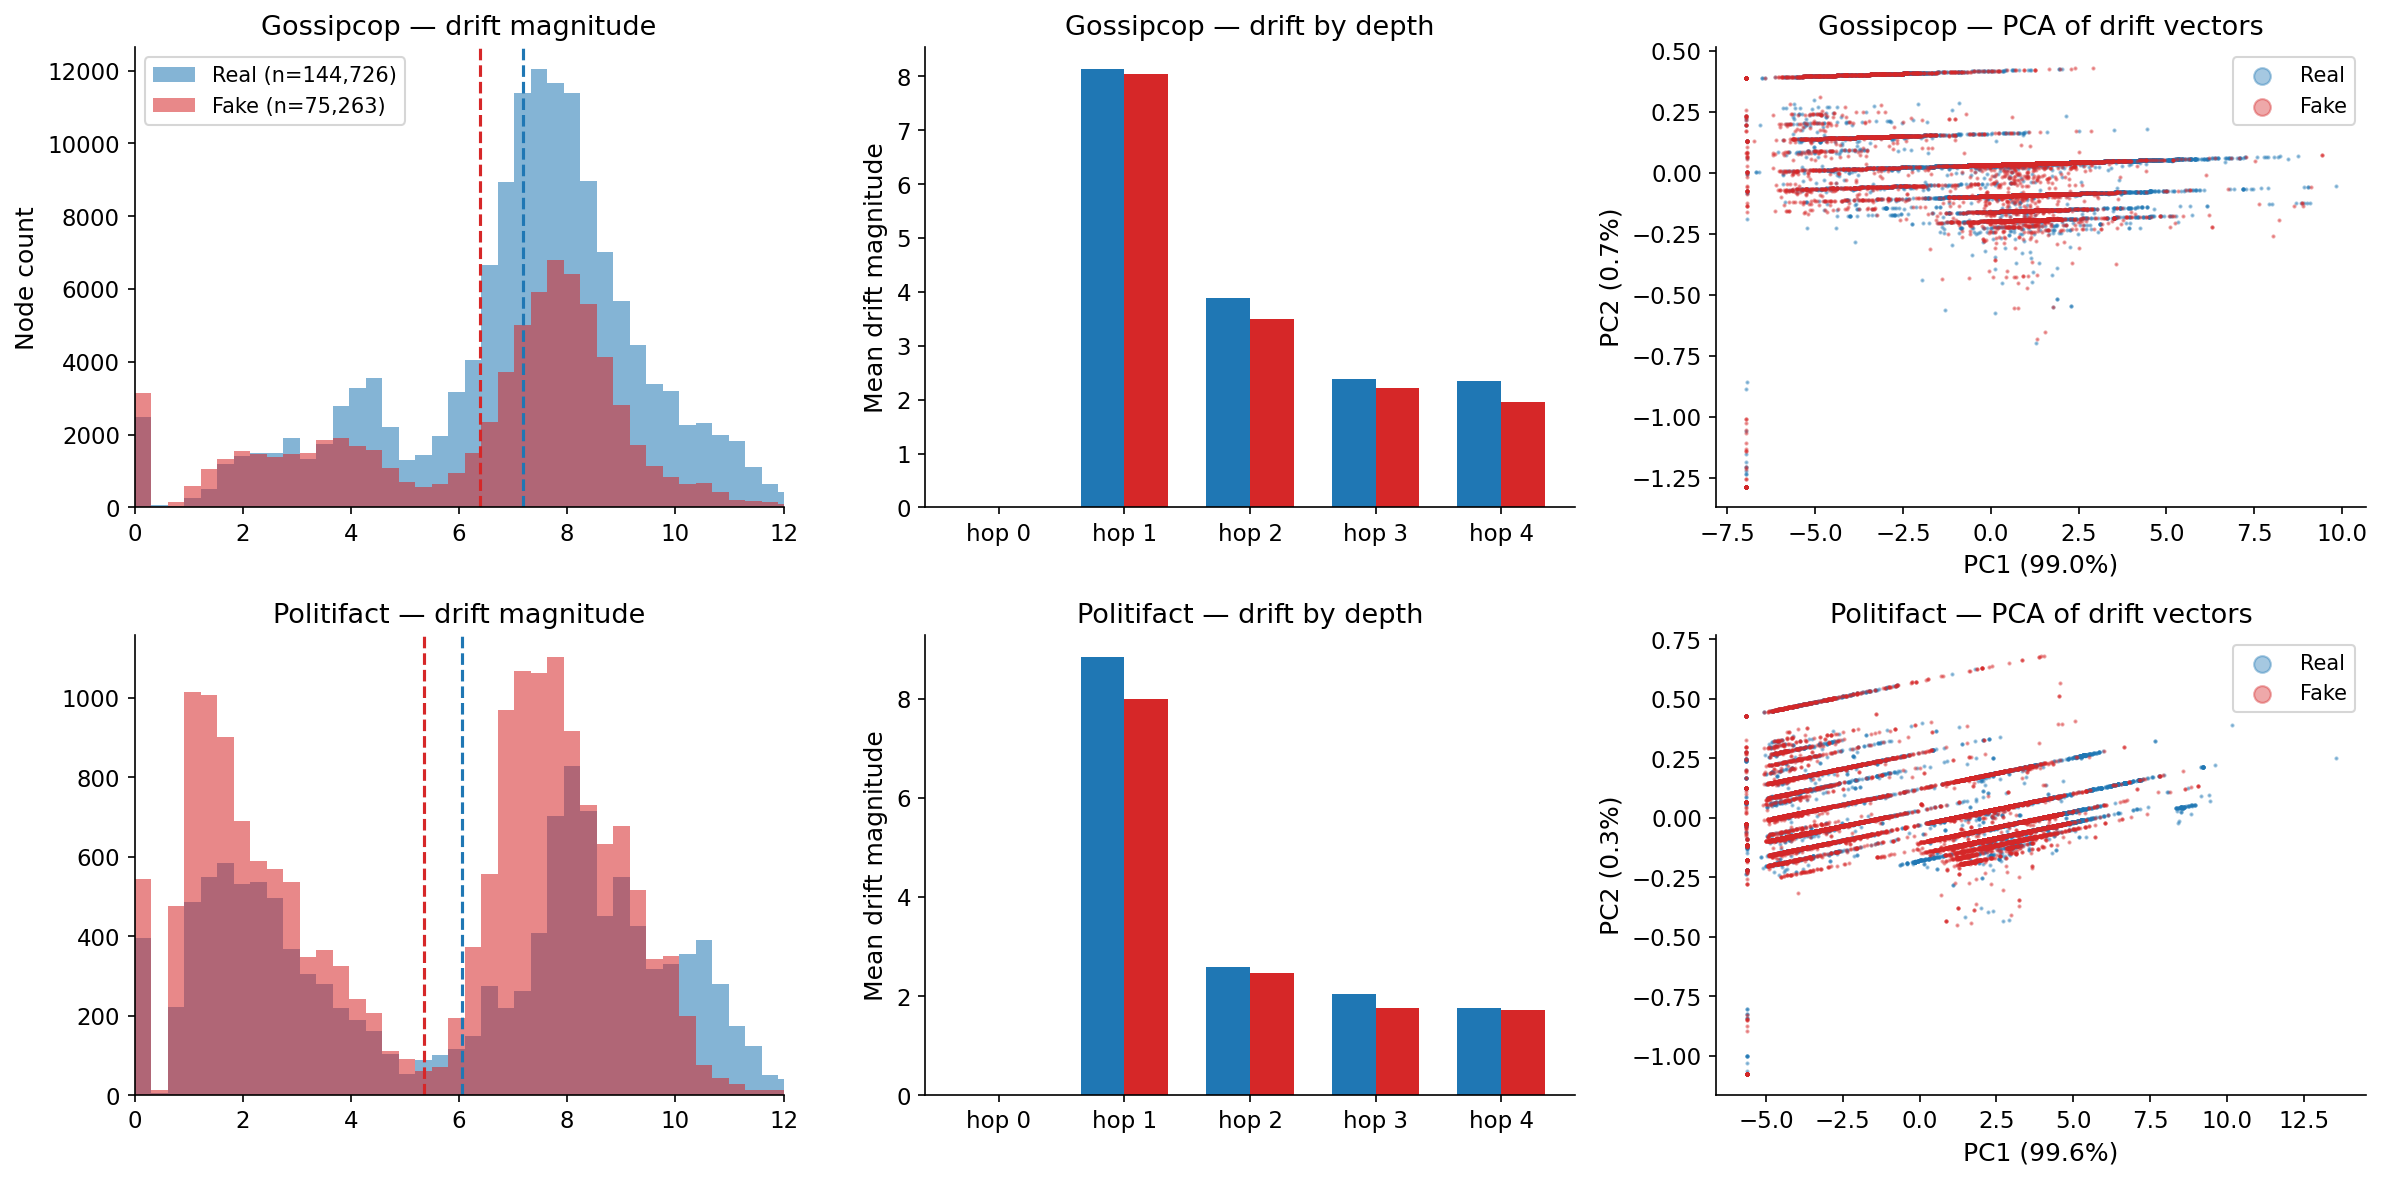
\includegraphics[width=\columnwidth]{../figures/drift_analysis.png}
  \caption{Drift analysis on GossipCop (top) and PolitiFact (bottom): magnitude
  histograms (left), drift by propagation depth (middle), and PCA of drift
  vectors (right).}
  \label{fig:drift}
\end{figure}

We computed per-node drift (Eq.~\ref{eq:drift}, cosine and $\ell_2$ components)
over the entire test sets---$\sim$220k GossipCop nodes and $\sim$31k PolitiFact
nodes.

\begin{table}[t]
  \centering
  \caption{Drift ratio statistics (test nodes). Fake news drifts $\sim$11\%
  less than real news on both datasets.}
  \label{tab:drift}
  \small
  \begin{tabular}{lccccc}
    \toprule
    Dataset & Real & Fake & Ratio & Welch $t$ & $p$ \\
    \midrule
    GossipCop & 7.18 & 6.39 & \textbf{0.890} & $-66.4$ & $<10^{-16}$ \\
    PolitiFact & 6.05 & 5.35 & \textbf{0.885} & $-17.7$ & $6{\times}10^{-70}$ \\
    \bottomrule
  \end{tabular}
\end{table}

\textbf{Interpretation.} Fake news spreads with $\sim$11\% less content
degradation per hop (Table~\ref{tab:drift}, Figure~\ref{fig:drift}). The
per-depth analysis shows the effect emerges at hop $\ge 2$ and grows with depth;
root-node drift is zero by construction (masked) for both classes, ruling out a
trivial root-source effect. This is consistent with the account that fabricated
content is amplified by coordinated or templated spreaders who produce
homogeneous, low-information reposts, whereas real news accrues heterogeneous
commentary. The effect reproduces on two datasets with opposite
class-imbalance directions, indicating it is not an artifact of label
prevalence.

% ------------------------------------------------------------------
\subsection{Drift-only discrimination}
\label{sec:discrimresult}

\begin{figure}[t]
  \centering
  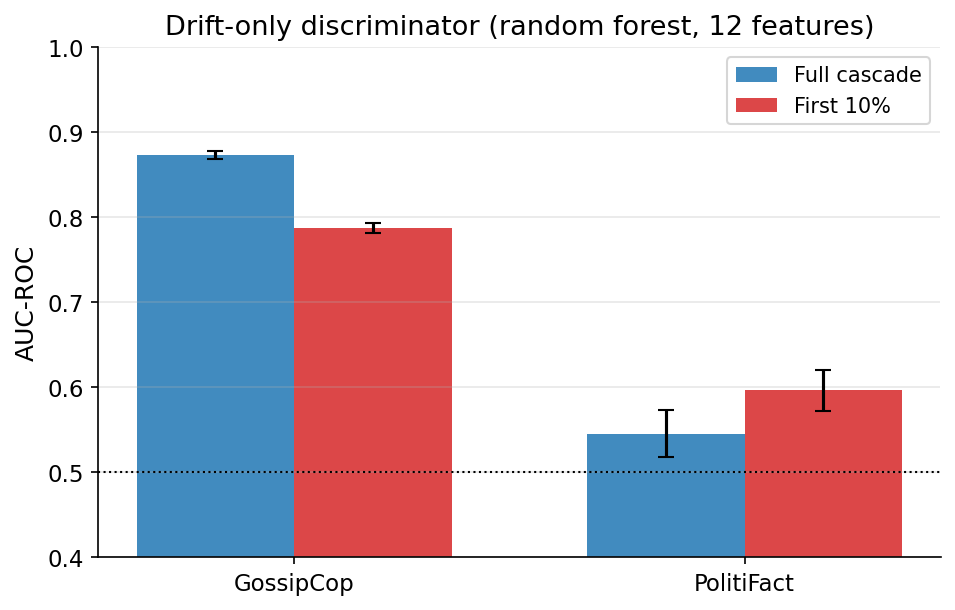
\includegraphics[width=\columnwidth]{../figures/discriminator.png}
  \caption{Drift-only discriminator (random forest, 12 features), full cascade
  vs.\ first 10\%, 5-fold cross-validated.}
  \label{fig:discrim}
\end{figure}

Using only the 12 graph-level drift statistics (no text, no neural network), a
random forest achieves the results in Table~\ref{tab:discrim} and
Figure~\ref{fig:discrim}.

\begin{table}[t]
  \centering
  \caption{Drift-only discrimination (5-fold CV means on the test split). The
  drift signal survives partial cascades.}
  \label{tab:discrim}
  \small
  \begin{tabular}{lcccc}
    \toprule
    Setting & \multicolumn{2}{c}{GossipCop} &
      \multicolumn{2}{c}{PolitiFact} \\
    \cmidrule(lr){2-3}\cmidrule(lr){4-5}
      & Acc & AUC & Acc & AUC \\
    \midrule
    Full cascade      & .795 & \textbf{.873} & .525 & .545 \\
    First 10\%        & .735 & \textbf{.787} & .558 & .597 \\
    \bottomrule
  \end{tabular}
\end{table}

The drift signal alone is strongly discriminative on GossipCop, and---importantly
---it \emph{survives partial cascades}: at 10\% of the cascade, drift-only still
yields 0.787 AUC, comparable to a fully-trained LSTM at 10\% truncation (78.7\%
accuracy). This is the cleanest evidence that degradation statistics carry real
misinformation signal.

% ------------------------------------------------------------------
\subsection{Ablation study}
\label{sec:ablation}

\begin{figure}[t]
  \centering
  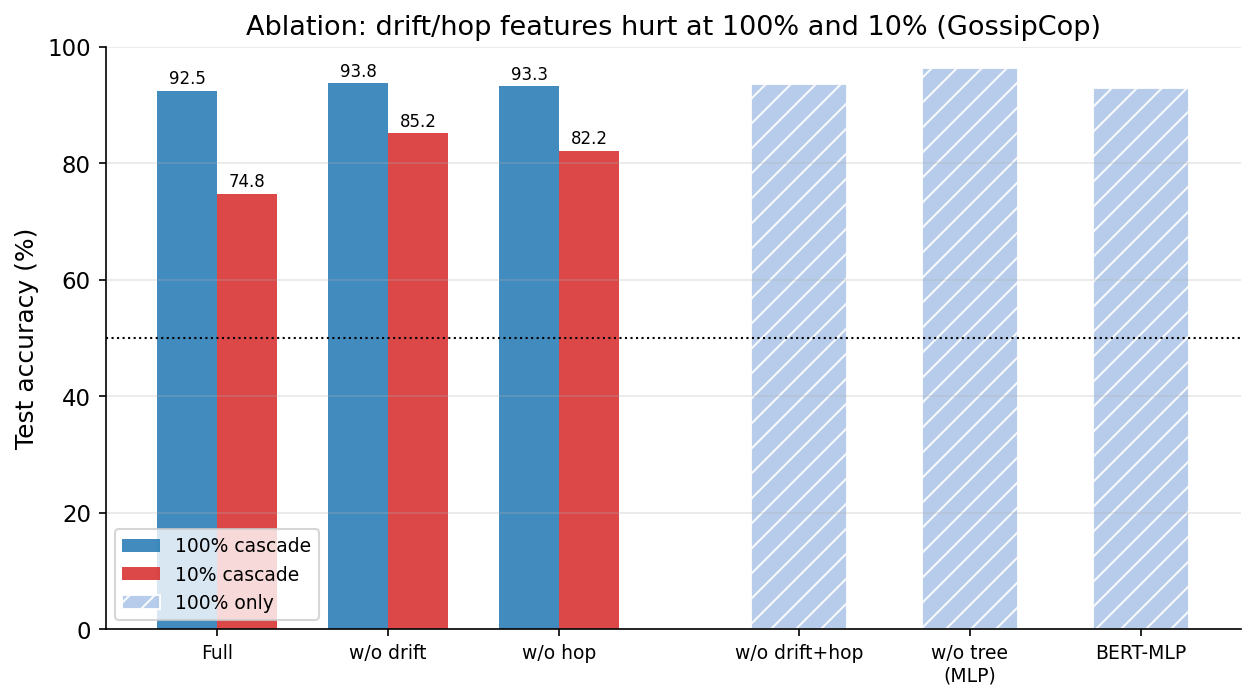
\includegraphics[width=\columnwidth]{../figures/ablation.png}
  \caption{Ablation of drift/hop features in DegradGNN at 100\% and 10\%
  cascade sizes (GossipCop).}
  \label{fig:ablation}
\end{figure}

\begin{table}[t]
  \centering
  \caption{Component ablation of DegradGNN (100\% data, single-run). Removing
  drift and hop features \emph{improves} accuracy.}
  \label{tab:ablation}
  \small
  \begin{tabular}{lcc}
    \toprule
    Variant & Accuracy & AUC \\
    \midrule
    Full (drift+hop+tree) & 0.9127 & 0.9688 \\
    w/o drift             & 0.9245 & 0.9743 \\
    w/o hop               & 0.9221 & 0.9737 \\
    w/o drift+hop         & 0.9334 & 0.9784 \\
    w/o tree (MLP)        & 0.9540 & 0.9797 \\
    BERT-MLP (text only)  & 0.9232 & 0.9704 \\
    \bottomrule
  \end{tabular}
\end{table}

\begin{table}[t]
  \centering
  \caption{Ablation re-run under partial cascades (seed 1). The ranking is
  consistent at 10\% truncation.}
  \label{tab:ablation10}
  \small
  \begin{tabular}{lcc}
    \toprule
    Variant & 100\% Acc & 10\% Acc \\
    \midrule
    Full      & 0.9247 & 0.7480 \\
    w/o drift & 0.9365 & \textbf{0.8521} \\
    w/o hop   & 0.9354 & 0.8220 \\
    \bottomrule
  \end{tabular}
\end{table}

\textbf{Finding.} Removing drift and hop features improves the model
(Tables~\ref{tab:ablation}, \ref{tab:ablation10}, Figure~\ref{fig:ablation}).
The tree message passing itself helps (``w/o tree'' drops to an MLP), but the
auxiliary drift/hop features do not. The honest conclusion: \emph{per-node
drift features are discriminative only in the aggregate; when injected into the
classifier they hurt at every cascade size.} This negative result reconciles the
strong drift-only discriminator (Section~\ref{sec:discrimresult}) with the
model-level ablation: the useful information is the \emph{distribution} of drift,
not its per-node instantiation.

% ------------------------------------------------------------------
\subsection{Partial-cascade (early detection) analysis}
\label{sec:early}

\begin{figure}[t]
  \centering
  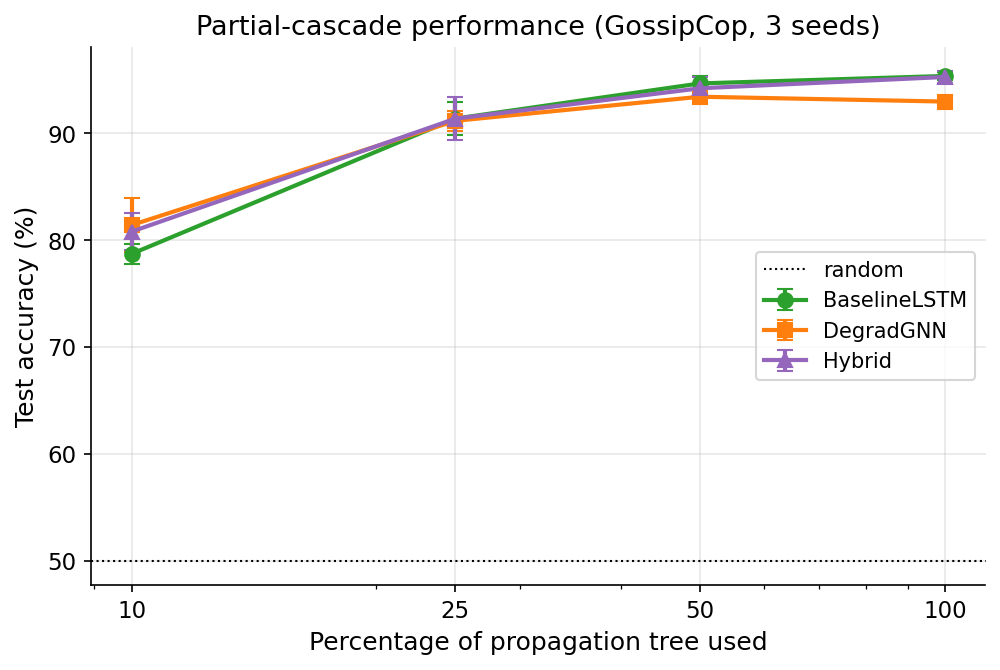
\includegraphics[width=\columnwidth]{../figures/early_detection.png}
  \caption{Partial-cascade performance on GossipCop (3 seeds, mean $\pm$ std):
  models trained on full cascades, tested on truncated cascades.}
  \label{fig:early}
\end{figure}

We evaluate models trained on full cascades against truncated test cascades
(keeping the shallowest fraction), 3 seeds (Figure~\ref{fig:early},
Table~\ref{tab:early}).

\begin{table}[t]
  \centering
  \caption{Multi-seed truncation results on GossipCop (accuracy, mean $\pm$
  std). All models degrade substantially at 10\%.}
  \label{tab:early}
  \small
  \begin{tabular}{lcccc}
    \toprule
    Model & 10\% & 25\% & 50\% & 100\% \\
    \midrule
    BaselineLSTM & .787$\pm$.010 & .914$\pm$.016 & .947$\pm$.007 & .954$\pm$.003 \\
    DegradGNN    & \textbf{.814}$\pm$.025 & .912$\pm$.009 & .934$\pm$.002 & .930$\pm$.004 \\
    HybridDegradLSTM & .808$\pm$.017 & .914$\pm$.020 & .942$\pm$.010 & .953$\pm$.005 \\
    \bottomrule
  \end{tabular}
\end{table}

All models degrade substantially when only 10\% of the cascade is available
(from $\sim$95\% to $\sim$79--81\%). Interestingly, the graph models (DegradGNN
81.4\%, Hybrid 80.8\%) are modestly \emph{more} robust to 10\% truncation than
the pure LSTM (78.7\%)---a $+2.5$ point mean gap---though per-seed variance
overlaps, so this is not significant at $n=3$. Consistent with the ablation,
per-node drift features do not confer truncation robustness. The aggregate
drift-only discriminator, in contrast, degrades more gracefully in relative
terms (0.873 $\rightarrow$ 0.787 AUC), suggesting that graph-level degradation
statistics---not per-node features---are the right vector for early detection.

% ==================================================================
\section{Discussion}
\label{sec:discussion}

% ------------------------------------------------------------------
\subsection{PolitiFact instability}
\label{sec:politifact}
With 62 training graphs, deep models on PolitiFact frequently collapse to the
majority class (48.9\%), and LSTM/Hybrid show $\pm$17\% variance across seeds.
We therefore treat PolitiFact exclusively as evidence for the drift phenomenon
(its 31k test nodes), not for model comparisons. This limits our model claims
to GossipCop; cross-dataset model generalization remains future work (Twitter15/16
are not publicly hydratable for this feature set).

% ------------------------------------------------------------------
\subsection{Statistical honesty}
\label{sec:stats}
\begin{itemize}[leftmargin=*,itemsep=2pt]
\item \textbf{Drift phenomenon:} robust, $n$ in the tens of thousands,
$p<10^{-70}$ on both datasets. This is our strongest claim.
\item \textbf{Hybrid vs.\ LSTM:} $+0.24\%$ accuracy and $+0.19\%$ AUC on
average, but $p=0.224$ / $0.452$ at $n=3$ seeds. The improvement is consistent
in direction (2/3 seeds positive in AUC) but we do \emph{not} claim it is
significant.
\item \textbf{Hybrid vs.\ DegradGNN:} $p=0.020$, Cohen's $d=3.98$---the LSTM
branch provides a significant gain over the GNN-only model.
\item We report mean $\pm$ std over seeds and exact per-seed values in
Appendix~\ref{app:perseed}, and note that MPS training is not bit-reproducible
even at a fixed seed.
\end{itemize}

% ------------------------------------------------------------------
\subsection{Why per-node drift hurts but aggregate drift helps}
\label{sec:why}
We hypothesize two mechanisms. (i) \textbf{Normalization shift:} drift features
are normalized per graph by current maxima; at truncation the depth/children
terms shift distribution, systematically misaligning the classifier's input.
(ii) \textbf{Signal-to-noise:} per-node drift is dominated by idiosyncratic
variation; only the aggregate moments (mean, std) separate the classes. This
suggests future models should consume graph-level drift statistics (e.g., via
set-pooling) rather than concatenating per-node drift.

% ==================================================================
\section{Conclusion}
\label{sec:conclusion}

We demonstrated that misinformation propagation leaves a measurable,
statistically robust signature: \textbf{fake news drifts $\sim$11\% less than
real news} ($p<10^{-70}$, two datasets). This signal is discriminative without
any text or graph features (0.873 AUC) and partially survives partial cascades
(0.787 AUC at 10\%). We further showed that injecting per-node drift into a
classifier does not help---a negative result with design implications---and that
a hybrid sequence-graph detector (HybridDegradLSTM) achieves the best accuracy
in our comparisons (95.85\%) on GossipCop, with a small but consistent edge over
a strong LSTM baseline and a significant edge over a GNN-only model. Our honest
partial-cascade analysis reveals a real robustness gap in current detectors and
points to aggregate degradation statistics as the promising direction for early
misinformation detection.

% ==================================================================
\begin{thebibliography}{9}
\small

\bibitem{dou2021upfd}
Y.~Dou, K.~Shu, C.~Xia, P.~S.~Yu, and L.~Sun.
\newblock User preference-aware fake news detection.
\newblock In \emph{Proceedings of the 44th International ACM SIGIR Conference on
Research and Development in Information Retrieval (SIGIR)}, 2021. (UPFD dataset.)

\bibitem{bian2020bigcn}
T.~Bian, X.~Xiao, T.~Xu, P.~Zhao, W.~Huang, Y.~Rong, and J.~Huang.
\newblock Rumor detection on social media with bi-directional graph
convolutional networks.
\newblock In \emph{AAAI Conference on Artificial Intelligence}, 2020.

\bibitem{kipf2017gcn}
T.~N.~Kipf and M.~Welling.
\newblock Semi-supervised classification with graph convolutional networks.
\newblock In \emph{International Conference on Learning Representations
(ICLR)}, 2017.

\bibitem{velickovic2018gat}
P.~Veli\v{c}kovi\'{c}, G.~Cucurull, A.~Casanova, A.~Romero, P.~Li\`{o}, and
Y.~Bengio.
\newblock Graph attention networks.
\newblock In \emph{International Conference on Learning Representations
(ICLR)}, 2018.

\bibitem{ma2016recurrent}
J.~Ma, W.~Gao, P.~Mitra, S.~Kwon, B.~J.~Jansen, K.-F.~Wong, and M.-Y.~Cha.
\newblock Detecting rumors from microblogs with recurrent neural networks.
\newblock In \emph{IJCAI}, 2016.

\bibitem{liu2018early}
Y.~Liu and Y.-F.~B.~Wu.
\newblock Early detection of fake news on social media through propagation
path classification with recurrent and convolutional networks.
\newblock In \emph{AAAI Conference on Artificial Intelligence}, 2018.

\bibitem{devlin2019bert}
J.~Devlin, M.-W.~Chang, K.~Lee, and K.~Toutanova.
\newblock BERT: Pre-training of deep bidirectional transformers for language
understanding.
\newblock In \emph{NAACL-HLT}, 2019.

\end{thebibliography}

% ==================================================================
\appendix
\section{Per-seed results (GossipCop)}
\label{app:perseed}

\begin{table}[h]
  \centering
  \caption{Per-seed accuracy and mean AUC-ROC on GossipCop.}
  \label{tab:appendix}
  \small
  \begin{tabular}{lccccc}
    \toprule
    Model & Seed 1 & Seed 2 & Seed 3 & Mean & Mean AUC \\
    \midrule
    GCN       & .7867 & .7804 & .7797 & .7823 & .8686 \\
    GAT       & .8973 & .9151 & .9158 & .9094 & .9646 \\
    BiGCN     & .9396 & .9375 & .9399 & .9390 & .9798 \\
    DegradGNN & .9328 & .9323 & .9247 & .9300 & .9780 \\
    BaselineLSTM & .9530 & .9556 & .9597 & .9561 & .9858 \\
    Hybrid    & .9543 & .9608 & .9605 & .9585 & .9876 \\
    \bottomrule
  \end{tabular}
\end{table}

\section{Reproducibility index}
\label{app:repro}
\begin{itemize}[leftmargin=*,itemsep=2pt]
\item \texttt{results/multiseed\_all.json} --- 3-seed main results (both datasets).
\item \texttt{results/significance.json} --- paired $t$-tests, Cohen's $d$, drift-ratio statistics.
\item \texttt{results/drift\_discriminator\_robustness.json} --- drift-only RF, full vs.\ 10\%, 5-fold.
\item \texttt{results/ablations.json}, \texttt{results/ablations\_10pct.json} --- ablations at 100\% and 10\%.
\item \texttt{results/early\_detection\_multiseed.json} --- multi-seed truncation curves.
\item \texttt{scripts/} --- \texttt{make\_figures.py}, \texttt{analysis\_stats.py},
  \texttt{run\_early\_detection.py}, \texttt{run\_ablation\_10pct.py},
  \texttt{run\_discriminator\_robustness.py}.
\item \texttt{figures/} --- all figures embedded above.
\end{itemize}

\emph{All experiments: Apple Silicon (MPS), PyTorch, PyG; one seed per process.}

\end{document}
